\documentclass[a4paper,% A4 papir size
                aps,% Document gets APS layout
                prl,% more layout, section numbering is removed
                amsfonts,% load AMS fonts
                amssymb,% load more AMS symboler
                amsmath,% load AMS math (equation environment and so on...)
                nobibnotes,% If BibTex is not used, REVTeX should be told to use normal footnotes
                twocolumn, % two-column layout
                twoside,% to-sided print
                balancelastpage,% balancing the last page when using two columns
                eqsecnum] % numbering the equations with the sectionnumber
                {revtex4-1}
\usepackage[utf8]{inputenc} % Correct formatting, makes danish letters available
\usepackage[english]{babel} % Language

% Place all other packages you use here i.e. graphicx, subfiles...
\usepackage{amsmath, amssymb}
\usepackage{url}
\usepackage{tabularx}
\usepackage{wrapfig}
\usepackage{subfiles}
% \usepackage[squaren]{SIunits}
\usepackage{siunitx}
\sisetup{per-mode=fraction,
        fraction-function=\tfrac,
        separate-uncertainty = true,
        % bracket-numbers = false,
        scientific-notation = true,
        uncertainty-separator = {\,}
      }
\usepackage{caption}
\captionsetup{labelfont={footnotesize,bf},textfont=footnotesize,format=hang,indention=-0.5cm} %makes nicer indents
\usepackage[normalem]{ulem}
\usepackage{subfigure}
\usepackage{lipsum}
\usepackage{todonotes}
\usepackage{booktabs}
\usepackage{microtype}
\begin{document} % Starts the actual document
\selectlanguage{english}

\title{Writing articles for Applied statistics \\ a \LaTeX
  template} % Title of the document, \\ can be used to generate linebreaks
\date{\today} % Date of the document, \today can be used

% Author on the articles. Add a new line of \author{Name} for each author
\author{Ammad Javaid Sheikh} \author{Lauge Emil Nielsen} \author{Oliver
  Christensen} \affiliation{Niels Bohr Institute - Applied statistics - Project
  1 group F14} % The authors affiliation

% With REVTeX the abstract must be before \maketitle
\begin{abstract}
  Measuring the gravitational acceleration $g$ to a high degree of precision is
  important for measuring force and physical quantities concerning a standard
  force. $g$ was measured using a simple pendulum setup and a ball rolling down
  an incline, with the aim to get $g$ to as high an accuracy and precision as
  possible. We found $g$ to be $9.81552 \pm 0.02723 \frac{m}{s^2}$ for the
  pendulum experiment, and ??? for the incline experiment, which was $0.020711$
  and ??? $\sigma$ in agreement with measurements by the Danish National Space
  Center, respectively. While we managed a high accuracy, our precision was less
  than ideal, partly due to the low number of measurements and being perhaps too
  cautious in our estimated errors.
\end{abstract}

\maketitle

% Resets the counters so references are logical:
\setcounter{section}{1} %Sets the sectioncounter to 1
\setcounter{equation}{0} %Sets the equationcounter to 0


% Begin the sections
% ------------------------------------------------------------------------------------------ %
\section{Introduction}
% ------------------------------------------------------------------------------------------ %
The gravitational acceleration $g$ is the acceleration on an object caused by
the force of gravitation. Having a precise value of $g$ is important for
measuring force and physical phenomena involving force, such as temperature (due
to the pressure dependence). In Copenhagen, this was calculated to be
$9.81546301 \pm 0.001 \frac{m}{s^2}$ in 2005 by the Danish National Space
Center.\cite{Gravity2005} In this project, we calculated $g$ using two methods,
one using a simple pendulum experiment and the other using a ball rolling down
an incline.

The aim of this project was to calculate the gravitational acceleration to as
high a precision and accuracy as possible, ideally a precision of less than one
part per thousand.

In order to get results of the desired accuracy and precision, the challenge
lies in getting accurate results and minimizing and propagating the
uncertainties.

\begin{figure*}[h]
  \centering, 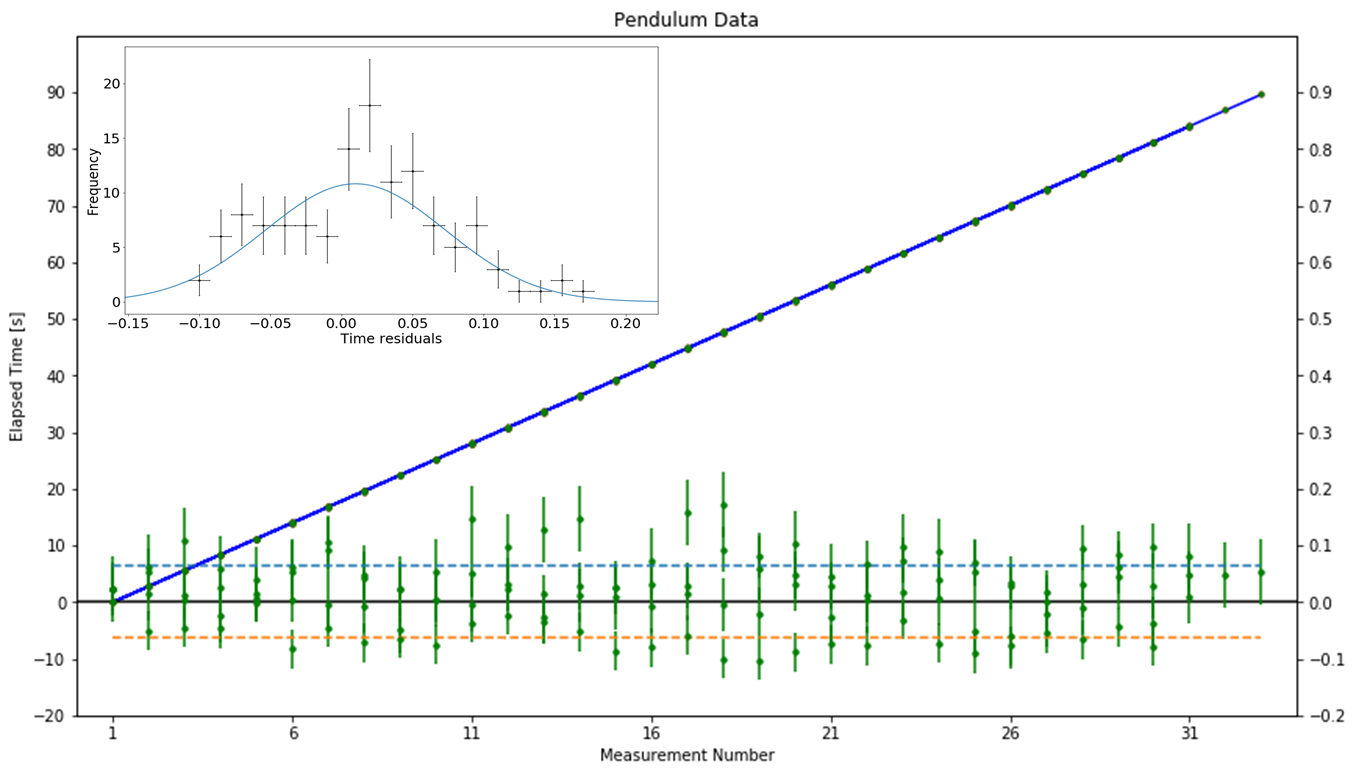
\includegraphics[width=\linewidth]{Picture1.png}
  \caption{Results of the fit for the period $T$ for 4 independent sequences of
    time measurements. The green dots are the measured periods; the blue line is
    the fit. Upper-left corner: Distribution of time residuals, assuming
    Gaussian distribution. Below: The line below shows the time residuals for
    the 4 sequences of measurements. The dashed lines show $\pm 1 \sigma$. The
    uncertainty on time measurements are obtained from the RMS of the
    differences in time measurements.}
  \label{fig:pendulumfit}
\end{figure*}

For the simple pendulum experiment, we measured the length $L$ and period $T$,
along with each group member's timing precision, to calculate $g$ using the
equation:
\begin{equation}
  g = L \left( \frac{2\pi}{T} \right)^2 \label{eq:Pendul}
\end{equation}

For the ball on incline experiment, we acceleration $a$, the radius of the ball
$R_{ball}$, the width of the rail $d_{rail}$ the angle of the incline with
respect to the table $\theta$ along with the angle of the table $\Delta \theta$.
$g$ was then calculated using the equation:

\begin{equation}
  g = \frac{a}{\sin(\theta + \Delta\theta)}\left[1+\frac{2}{5}\frac{R_{ball}^2}{R_{ball}^2 - (\frac{d_{rail}}{2})^2}\right] \label{eq:Ball}
\end{equation}

The errors on $g$ were in each experiment calculated using standard error
propagation:

\begin{equation}
  \sigma^2_y = \sum\limits_{i,j}^n
  \left \{ \frac{\delta y}{\delta x_i} \frac{\delta y}{\delta x_j} \right \} V_{ij}
\end{equation}

where $V$ is the covariance matrix.


% ------------------------------------------------------------------------------------------ %
\section{Method}
\subsection{Simple pendulum}



The pendulum length $L$ we defined as the length from the top of the hook to the
middle of the weight. $L$ was measured using both a ruler and a laser in order
to cross-check results. For the ruler, it was not long enough to calculate the
length in one go, for which $L$ was combined using several measurements. For the
laser, it only measures the length from floor to ceiling, by which $L$ needs to
be determined by subtracting the length from floor to middle of weight, along
with the length from ceiling to hook, measured using the ruler. Errors for $L$
were determined using addition error propagation.

$L$ was measured in a total of 4 ways. (a) As the length from the top of the
hook to the top of the weight plus half the difference between the position of
the top to the bottom of the weight. (b) As the length from the top of the hook
to the bottom of the weight minus half the difference between the position of
the top to the bottom of the weight. (c) From the ceiling to the top of the
weight minus the distance from the ceiling to the top of the hook plus half the
difference between the position of the top to the bottom of the weight. (d) With
the laser, from the ceiling to the floor, minus the length from the floor to the
middle of the weight and the length from ceiling to hook, measured using the
ruler.

The period was determined by putting a box diagonally to the pendulum and taking
one lap when the pendulum appears from behind the box. Individual timing
precision was estimated by measuring each group member's consistency in being
able to press Enter.

\subsection{Ball rolling down incline}
The rail width $d_{rail}$ and ball radius $R_{ball}$ were measured using a
caliper, one with a precision of 0.01 mm and one with a precision of 0.1 mm.

$\theta$ was calculated using both a protractor and by calculating it from the
length and height of the incline measured using a ruler, then getting the angle
via Pythagoras' equation. $\Delta \theta$ was calculated by turning the
experimental setup 180 degrees and measuring $\theta$, along with the incline
length and height again. As the value should be $\theta + \Delta \theta$ for one
side and $\theta - \Delta \theta$ for the other, the difference between the
measurements should be equal to $2 \Delta \theta$.

The acceleration $a$ was obtained by measuring the gate positions on the incline
and times when the ball passes through the gate in order to get the acceleration
$a$ (assumed constant) using a quadratic fit. One value for $a$ was obtained for
each of the the $2*15$ data sets – half of which were measured after rotations
of the experimental setup. The error on each acceleration was determined through
error propagation of the errors of distance measurements (measured with a
ruler). Our estimation of the true acceleration is then the weighted average of
these values, resulting in ### for the first 15 measurements and ### for the
last 15 measurements.

The times when the ball passes the gates were captured using the program
Waveforms, with a rate of $5kHz$.

The acceleration was obtained by performing a quadratic fit on the data points
(Time [s], Position [m]). One value for a was obtained for each of the the 2 *
15 data sets – half of which were measured after rotations of the experimental
setup. The error on each acceleration was determined through error propagation
of the errors of distance measurements (measured with a ruler). Our estimation
of the true acceleration is then the weighted average of these values, resulting
in ### for the first 15 measurements and ### for the last 15 measurements.


% ------------------------------------------------------------------------------------------ %
\section{Results}
\subsection{Pendulum}

%% Table for Pendulum
\begin{table}[h]
  \caption{Pendulum experiment: list of variables used for determining $g$,
    their uncertainties and their impact on $g$.}
  \centering
  \begin{tabular}{lccc}
    Parameter & Mean $\mu$ &  $\hat{\sigma}_{\mu}$ &  Impact on $g$ \\\toprule
    Length $L$ (Ruler) [\si{\m}] & \num[round-precision=6,round-mode=figures]{1950.73} & \num[round-precision=5,round-mode=figures]{0.19248} & \num[round-precision=5,round-mode=figures]{0.00096850} \\
    Period $T$ [\si{\s}]  & \num[round-precision=6,round-mode=figures]{2.80209} & \num[round-precision=5,round-mode=figures]{0.00042782} & \num[round-precision=5,round-mode=figures]{0.027242} \\
    Length $L$ (Laser) [\si{\m}] & \num[round-precision=6,round-mode=figures]{1950.56} & \num[round-precision=5,round-mode=figures]{0.57849} & \num[round-precision=5,round-mode=figures]{0.0029108} \\
    Impact for $T$  & \num[round-precision=6,round-mode=figures]{} & \num[round-precision=5,round-mode=figures]{} & \num[round-precision=5,round-mode=figures]{0.027240} \\
    Length $L$ (All) [\si{\m}] & \num[round-precision=6,round-mode=figures]{1950.71} & \num[round-precision=5,round-mode=figures]{0.18263} & \num[round-precision=5,round-mode=figures]{0.00091897} \\
    Impact for $T$  & \num[round-precision=6,round-mode=figures]{} & \num[round-precision=5,round-mode=figures]{} & \num[round-precision=5,round-mode=figures]{0.027242} \\
  \end{tabular}
\end{table}

For the pendulum experiment, $g$ was measured to be $9.81543 \pm 0.02723
\frac{m}{s^2}$, using all measurements. For the three ruler measurements only,
$g = 9.81552 \pm 0.02723 \frac{m}{s^2}$. For the laser measurement only, $g =
9.81467 \pm 0.02740 \frac{m}{s^2}$. While our accuracy is good, our precision is
not particularly high, which is primarily due to the error on our period
measurements. As can be seen in Table I, the period's impact on $g$ is much
larger than that of $L$.

Figure 1 shows

Comparing our found values for $g$ to the one found by the Danish National Space
Center, we get a z-score of $z = 0.020711$ using all data, $z = 0.040567$ using
only the ruler data, and $z = 0.25743$ using only the laser data. Comparing the
ruler data and laser data, we see that $g$ for the laser data is further away
from the "true" value, which is likely due to our measurement from the floor to
the bottom of the weight, as the laser itself should be accurate, and this is
the only other value not used in the other length measurements.

The measurements of the pendulum length calculated from the top of the hook to
the top of the weight plus the middle of the weight. We decided not to include
the ruler measurements from the ceiling to the top of the hook, due to
disagreement with the other measurements and relatively high uncertainty due to
addition error propagation, as it requires the combination of several
measurements.

\subsection{Ball on an incline}
\sisetup{round-precision=4, round-mode=figures}
\begin{table}
  \begin{tabularx}{\linewidth}{*{2}X @{~$\pm$~} *{2}X}
    Parameter & Mean $\mu$ & $\hat{\sigma}_{\mu}$ & Impact on $g$ \\\cmidrule{1-4}
    $a_{\mathrm{fw}}$ $\left[\si{\m\per\s\squared}\right]$ & \num{1.520936084321771} & \num{0.002048096350081636}  & \num{0.0033486314209362953 } \\ 
    $\theta$ [\si{\degree}] & \num[scientific-notation=false]{13.519782107715763} & \num{0.018965252051556677}   & \num{0.01725824805265002   } \\
    $\Delta\theta$ [\si{\degree}] & \num[scientific-notation=false]{0.26658053316106} & \num{0.012319922605459792}   & \num{0.011211044268563961 }  \\ 
    $R_{\mathrm{ball}}$ [\si{\m}] & \num{0.006351119402985075} & \num{2.4937733402690825e-06} & \num{0.00023054486627327155} \\ 
    $d_{\mathrm{rail}}$ [\si{\m}] & \num{0.0063881422924901175} & \num{4.445542244743871e-06}  & \num{0.00040860052103689637}
  \end{tabularx}
\end{table}

For the ball-on-incline experiment, we measured $g$ to be $\SI{9.79963 \pm
  0.020855}{\m\per\s\squared}$.


% ------------------------------------------------------------------------------------------ %
\section{Discussion}

% ------------------------------------------------------------------------------------------ %
\section{Conclusion}

In conclusion, the gravitational acceleration $g$ was measured using both a
simple pendulum and a ball on incline setup.

% ------------------------------------------------------------------------------------------ %
\begin{thebibliography}{99}
  % Literature you can refer to
\bibitem{Griffiths} D. J. Griffiths, \emph{Introduction to Electrodynamics 3.
    edition}, (Pearson Education, Inc. 1999)
\bibitem{Gravity2005} Strykowski et al., \emph{Gravity measurements in Denmark
    in 2005}, (Danish National Space Center, Technical Report No. 6, May 2006)
\end{thebibliography}

\end{document} % Slut på dokument, alt herefter ignoreres
